\chapter{Implementation}
\label{ch:impl}
\chaptermark{Fourth Chapter Heading}

\definecolor{codegreen}{rgb}{0,0.6,0}
\definecolor{codegray}{rgb}{0.5,0.5,0.5}
\definecolor{codepurple}{rgb}{0.58,0,0.82}
\definecolor{backcolour}{rgb}{0.95,0.95,0.92}
\definecolor{light-gray}{gray}{0.95}

\newcommand{\code}[1]{\colorbox{light-gray}{\texttt{#1}}}

\lstdefinestyle{mystyle}{
    caption=Example C++,
    label={lst:listing-cpp},
    language=C++,
    backgroundcolor=\color{backcolour},
    commentstyle=\color{codegreen},
    keywordstyle=\color{magenta},
    numberstyle=\tiny\color{codegray},
    stringstyle=\color{codepurple},
    basicstyle=\ttfamily\footnotesize,
    breakatwhitespace=false,
    breaklines=true,
    keepspaces=true,
    numbers=left,
    numbersep=5pt,
    showspaces=false,
    showstringspaces=false,
    showtabs=false,
    tabsize=2,
}
\lstset{style=mystyle}


The following chapter provides implementation details for the system, including some issues that arose during development and the solutions to these issues.


\section{Implementation of Load generation module}\label{sec:yandex_tank_use}
Yandex Tank~\cite{yandex_tank} is used as the main load generation tool for my system. It supports many load generation engines, but I chose Phantom~\cite{phantom} as the primary engine. Phantom only supports HTTP~\cite{http} requests and can be configured in two ways
\begin{itemize}
    \item Single configuration file. This type of configuration is convenient to store, but it only supports HTTP GET~\cite{http} method.
    \item Configuration file and ammo file. For more complex scenarios with all types of HTTP methods, Phantom~\cite{phantom} suggests to use ammo file. Ammo file contains a sequence of HTTP requests.
\end{itemize}
Yandex Tank has built-in integration with InfluxDB~\cite{influxdb} and is able to directly write all test results to it.
Yandex Tank API~\cite{yandex_tank_api} is a web server that incapsulates work with Yandex Tank using REST API. It is used as an implementation of the load generation module.


\section{Implementation of configuration manager module}
Consul~\cite{consul} is an open-source solution for automating service configuration and discovery. It is used as a configuration manager due to its key/value storage feature. It provides a REST API for managing key/value storage, and most importantly, Watches~\cite{consul_watches}, which allows all services integrated with Consul to be notified of any changes to configs. It allows to track the impact of configuration changes during load testing. Example in Section ~\ref{example???} demonstrates this in realistic conditions.


\section{Datastore}\label{sec:implementation-of-datastore}
Datastore is divided into two parts:

\subsection{PostgreSQL}\label{subsec:postgresql}
PostgreSQL~\cite{postgresql} is a powerful, open-source object-relational database management system. It is used as the main storage for testing scenarios and metadata about their executions. Figure~\ref{fig:erd} shows the entity-relationship diagram of the database schema.
\begin{figure}[t]
    \centering
    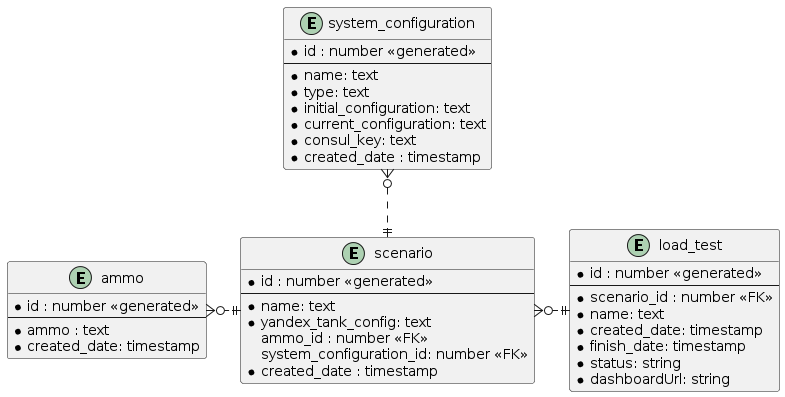
\includegraphics[height=\textheight,width=\textwidth,keepaspectratio]{erd.png}
    \caption{Entity-Relationship Diagram}
    \label{fig:erd}
\end{figure}

Scenarios are stored in three tables:
\begin{itemize}
    \item \code{scenario} table stores the main information about scenario
    \item \code{system\_configuration} table contains the configuration of the tested system and the key to the Consul key/value storage used to manage the configurations. The initial configuration is the configuration that the system needs at the start of a test, while the current configuration refers to configuration in real time.
    \item \code{ammo} table stores ammo configurations. Ammo is a special term used in Yandex Tank~\cite{yandex_tank}, which is explained in Subsection~\ref{sec:yandex_tank_use}
\end{itemize}
System configurations and ammo are allocated in separate tables, as we have a one-to-many relationship (several scenarios may have the same configuration and ammo), and such a relationship should be represented in the form of separate tables to avoid unnecessary data repetitions~\cite{normal_forms}.

Table \code{load\_test} stores metadata about the executions with the following attributes:
\begin{itemize}
    \item Created and finish date of the execution.
    \item Name of the specific execution.
    \item Status of the execution. Status can be: created, locked, running,  stopped,  failed, finished, starting.
    \item Dashboard URL to the visualization the results of the tests.
    \item ID for unique identification execution and map it to results
    \item Scenario ID for the linking execution with its scenario.
\end{itemize}

\subsection{InfluxDB}\label{subsec:influxdb}
InfluxDB~\cite{influxdb} is an open-source time series database management system. It is used as the main storage for the results of tests, which are stored as following time series:
\begin{itemize}
    \item Response time aggregated with the following quantiles: 100, 99, 95, 90, 75, and 50
    \item Number of threads needed to support a set RPS
    \item Number of responses aggregated with HTTP and Net codes. Net codes are standard codes from POSIX~\cite{posix_errors} used to signal problems with the network.
\end{itemize}


\section{Implementation of Orchestrator module}\label{sec:ochestrator_impl}
Orhestrator module was implemented using Orchestrator microservice. I implement it using Kotlin~\cite{kotlin} programming language and Spring framework~\cite{spring} for web development. Hibernate~\cite{hibernate} is Java library for constructing object-relationship mapping between Java objects and Database. I used it for communication with the PostgreSQL service. Additionally, Orchestrator service was integrated with Yandex Tank API and Consul service.

\subsection{REST API}\label{subsec:rest_api}
Orchestrator service provides an REST API for creating and managing ammo files, system configurations, scenarios, and load tests
Table~\ref{tab:rest_api_scenario} provides an example of REST API for scenarios.
\begin{longtable}[c]{|p{2cm}|p{5.5cm}|p{2.5cm}|p{5cm}|}
    \caption{REST API for scenarios}
    \label{tab:rest_api_scenario} \\
    \hline    \textbf{HTTP Method} & \textbf{URL} & \textbf{Body} & \textdf{Description} \\
    \endhead    \hline    POST & /api/scenario?name=<> & text/plain & Method for creating a scenario. Accept YAML~\cite{yaml} config in the body \\
    \hline    DELETE & /api/scenario?id=<key> & - & Method for deleting a scenario. All tests with this scenario will be stopped and deleted \\
    \hline    GET & /api/scenario/<id> & - & Method for getting the scenario by its id
    \hline    GET & /api              & - & Method for getting all scenarios
    \hline
\end{longtable}

\subsection{Integration with Yandex Tank API}\label{subsec:yandex_tank_api_integration}
First of all, Orchestrator service needed to be able to use load testing tool. I implemented an integration with Yandex Tank API using its REST API. Yandex Tank API stores only information about status of the test, and all other information is stored in PostgreSQL table \code{load\_test}. Figure~\ref{fig:creation} illustrates the example of starting the test.
\begin{figure}[t]
    \centering
    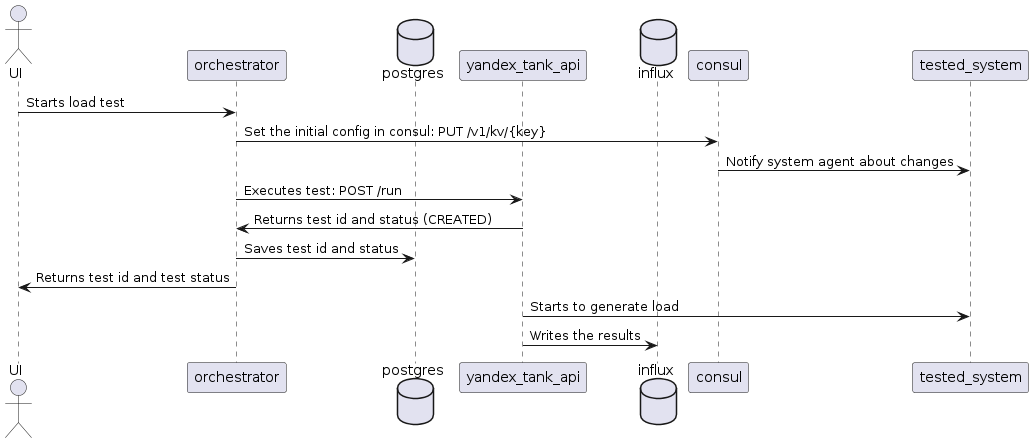
\includegraphics[height=\textheight,width=\textwidth,keepaspectratio]{creation.png}
    \caption{Example of starting the test}
    \label{fig:creation}
\end{figure}

\subsection{Integration with Consul}\label{subsec:consul_integration}
Consul key/value storage provides an REST API for managing the configurations. I used this API to read and update configurations in Consul.

\subsection{Polling mechanism}\label{subsec:polling_mechanism}
To have an actualized status of the load test and configuration of the system, I used http short polling strategy~\cite{http_polling}.
Figure~\ref{fig:polling} illustrates the process. Every three seconds, I poll the statuses and system configurations of unfinished tests and actualize them.
For this purpose, I used a Spring mechanisms for scheduling tasks. The code of the polling mechanism is presented in Listing~\ref{lst:polling}.
\begin{figure}[t]
    \centering
    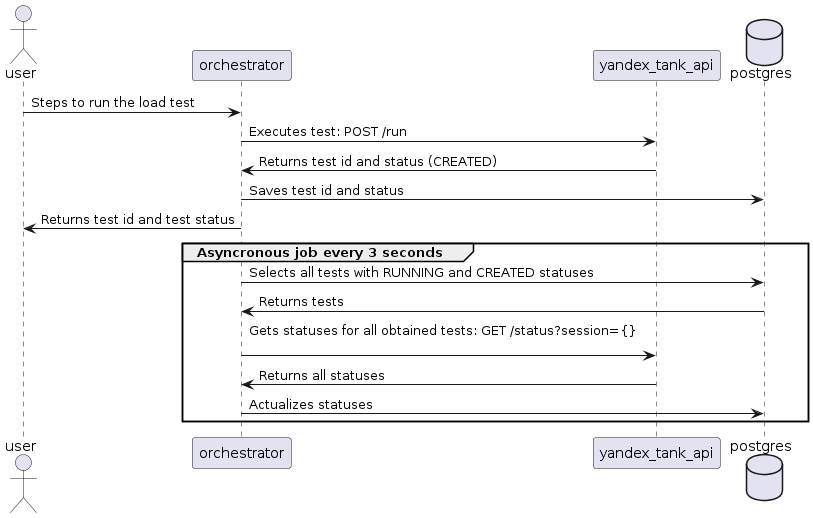
\includegraphics[height=\textheight,width=\textwidth,keepaspectratio]{polling.png}
    \caption{Polling mechanism}
    \label{fig:polling}
\end{figure}

\lstinputlisting[language=Kotlin, caption=Polling function, label={lst:polling}]{code/polling.kt}


\section{Implementation of UI}\label{sec:implementation-of-ui}
It was necessary to visualize scenario data and launch results.
Subsection~\ref{subsec:visualization-of-the-results} presents solution for the visualization of the results using Grafana.
Subsection~\ref{subsec:ui-of-the-orchestrator} provides an implementation for the visualizing other parts of the orchestrator.
\subsection{Visualization of the results}\label{subsec:visualization-of-the-results}
The default way of visualizing the results of the Yandex Tank is Overload service~\cite{overload}. It is the distinct web service that store and visualize the results. The problem with using it is the immutability of the UI. Therefore, I used the Grafana tool~\cite{grafana} and implemented a custom dashboard for visualization that can be easily modified through the UI of the Grafana. Figure~\ref{fig:grafana} demonstrates an example of the results on my dashboard.
\begin{figure}[t]
    \centering
    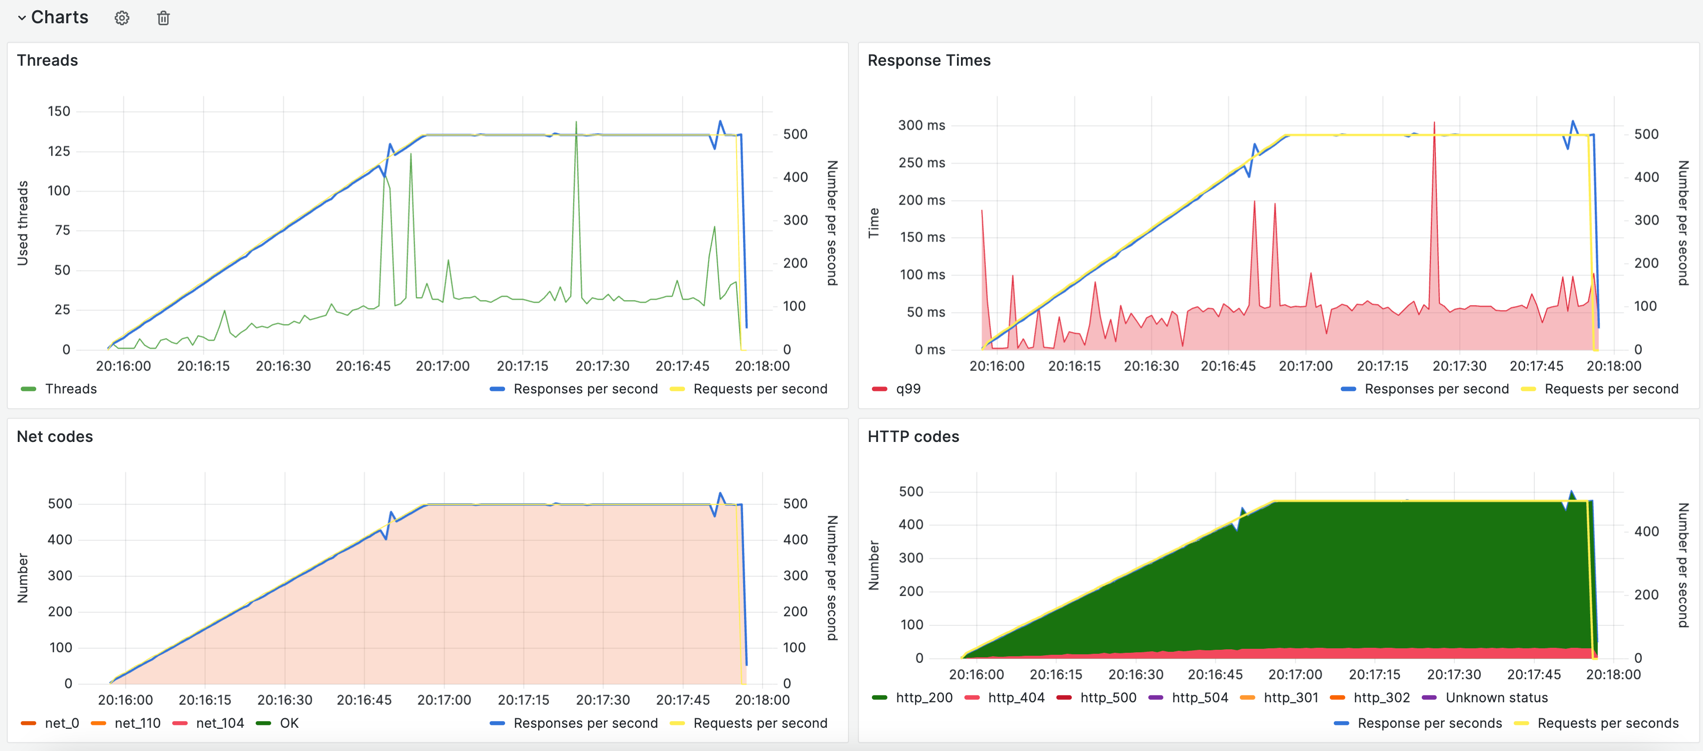
\includegraphics[height=\textheight,width=\textwidth,keepaspectratio]{grafana.png}
    \caption{Example of the charts in Grafana}
    \label{fig:grafana}
\end{figure}

\subsection{UI of the orchestrator}\label{subsec:ui-of-the-orchestrator}
Orchestrator needs a user interface for more convenient use of the service. Vaadin~\cite{vaadin} is a web application platform that allows developers to create an UI using Kotlin. It incapsulates all front-end development in Kotlin objects. For Orchestrator I developed four views: load tests, scenarios, ammo, and system configurations. Each view contains a table with the data, search field, and a creation form. Figures~\ref{fig:ui} and~\ref{fig:form} demonstrates examples of this views.\begin{figure}[t]
    \centering
    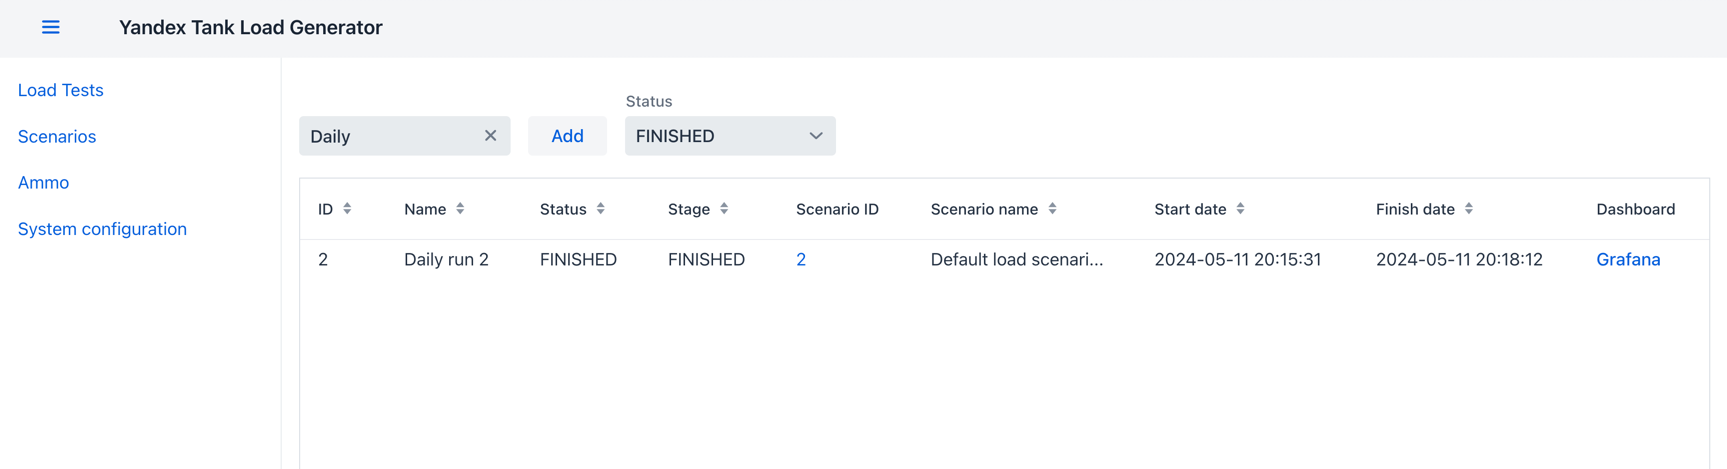
\includegraphics[height=\textheight,width=\textwidth,keepaspectratio]{ui.png}
    \caption{Example of the UI of the orchestrator}
    \label{fig:ui}
\end{figure}
\begin{figure}[t]
    \centering
    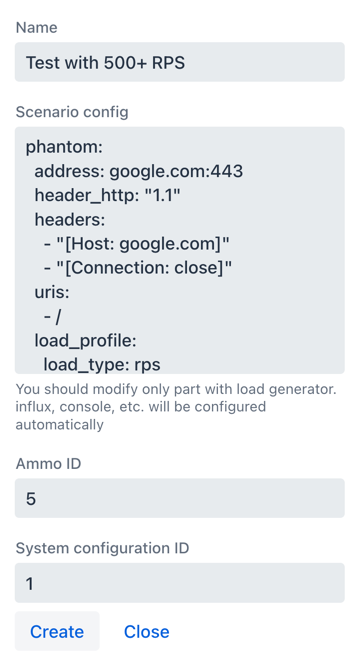
\includegraphics[height=\textheight,width=\textwidth,keepaspectratio]{creation_form.png}
    \caption{Form for creation scenarios}
    \label{fig:form}
\end{figure}

\subsection{Infrastructure}\label{subsec:infrastructure}
Docker~\cite{docker} image is a lightweight, standalone, and executable package that contains everything needed to run an application, including the code, runtime, libraries, and system tools. Docker container is an instance of a Docker image that is running in isolation on a host operating system.
For easier deployment and management of the described services, each service has been packaged into a Docker image. Grafana, Consul, InfluxDB and PostgreSQL services already have built images, but Yandex Tank API and Orchestrator need to be built. For the Yandex Tank API image I used the default image of Yandex Tank~\cite{yandex_tank_image} as based image, then tuned the system parameters for better performance, installed all dependencies, and ran the Yandex Tank API server. For Orchestrator, I first built a JAR file for my project using Gradle~\cite{gradle}, and then using a base image with the Java Runtime Environment installed, execute the compiled JAR file.

Then to orchestrate all containers and network between them, I used the Docker Compose tool~\cite{docker_compose}, which allows to describe all containers in a single YAML~\cite{yaml} file. Listing~\ref{lst:docker_compose} illustrates a part of this file for Orchestrator and PostgreSQL containers.
\lstinputlisting[language=Octave, caption=Part of the Docker Compose file, label={lst:docker_compose}]{code/docker-compose.yaml}.

\section{Conclusion}\label{sec:conclusion}
The system is implemented using the Yandex Tank API, Consul, Grafana, PostgreSQL, and InfluxDB tools. The Orchestrator web service was developed using Kotlin and Spring. Additionally, all the services was packed into Docker images, and the infrastructure of the application was up using these images with Docker Compose.
Figure~\ref{fig:architecture} shows the final architecture of the system.

\begin{figure}[t]
    \centering
    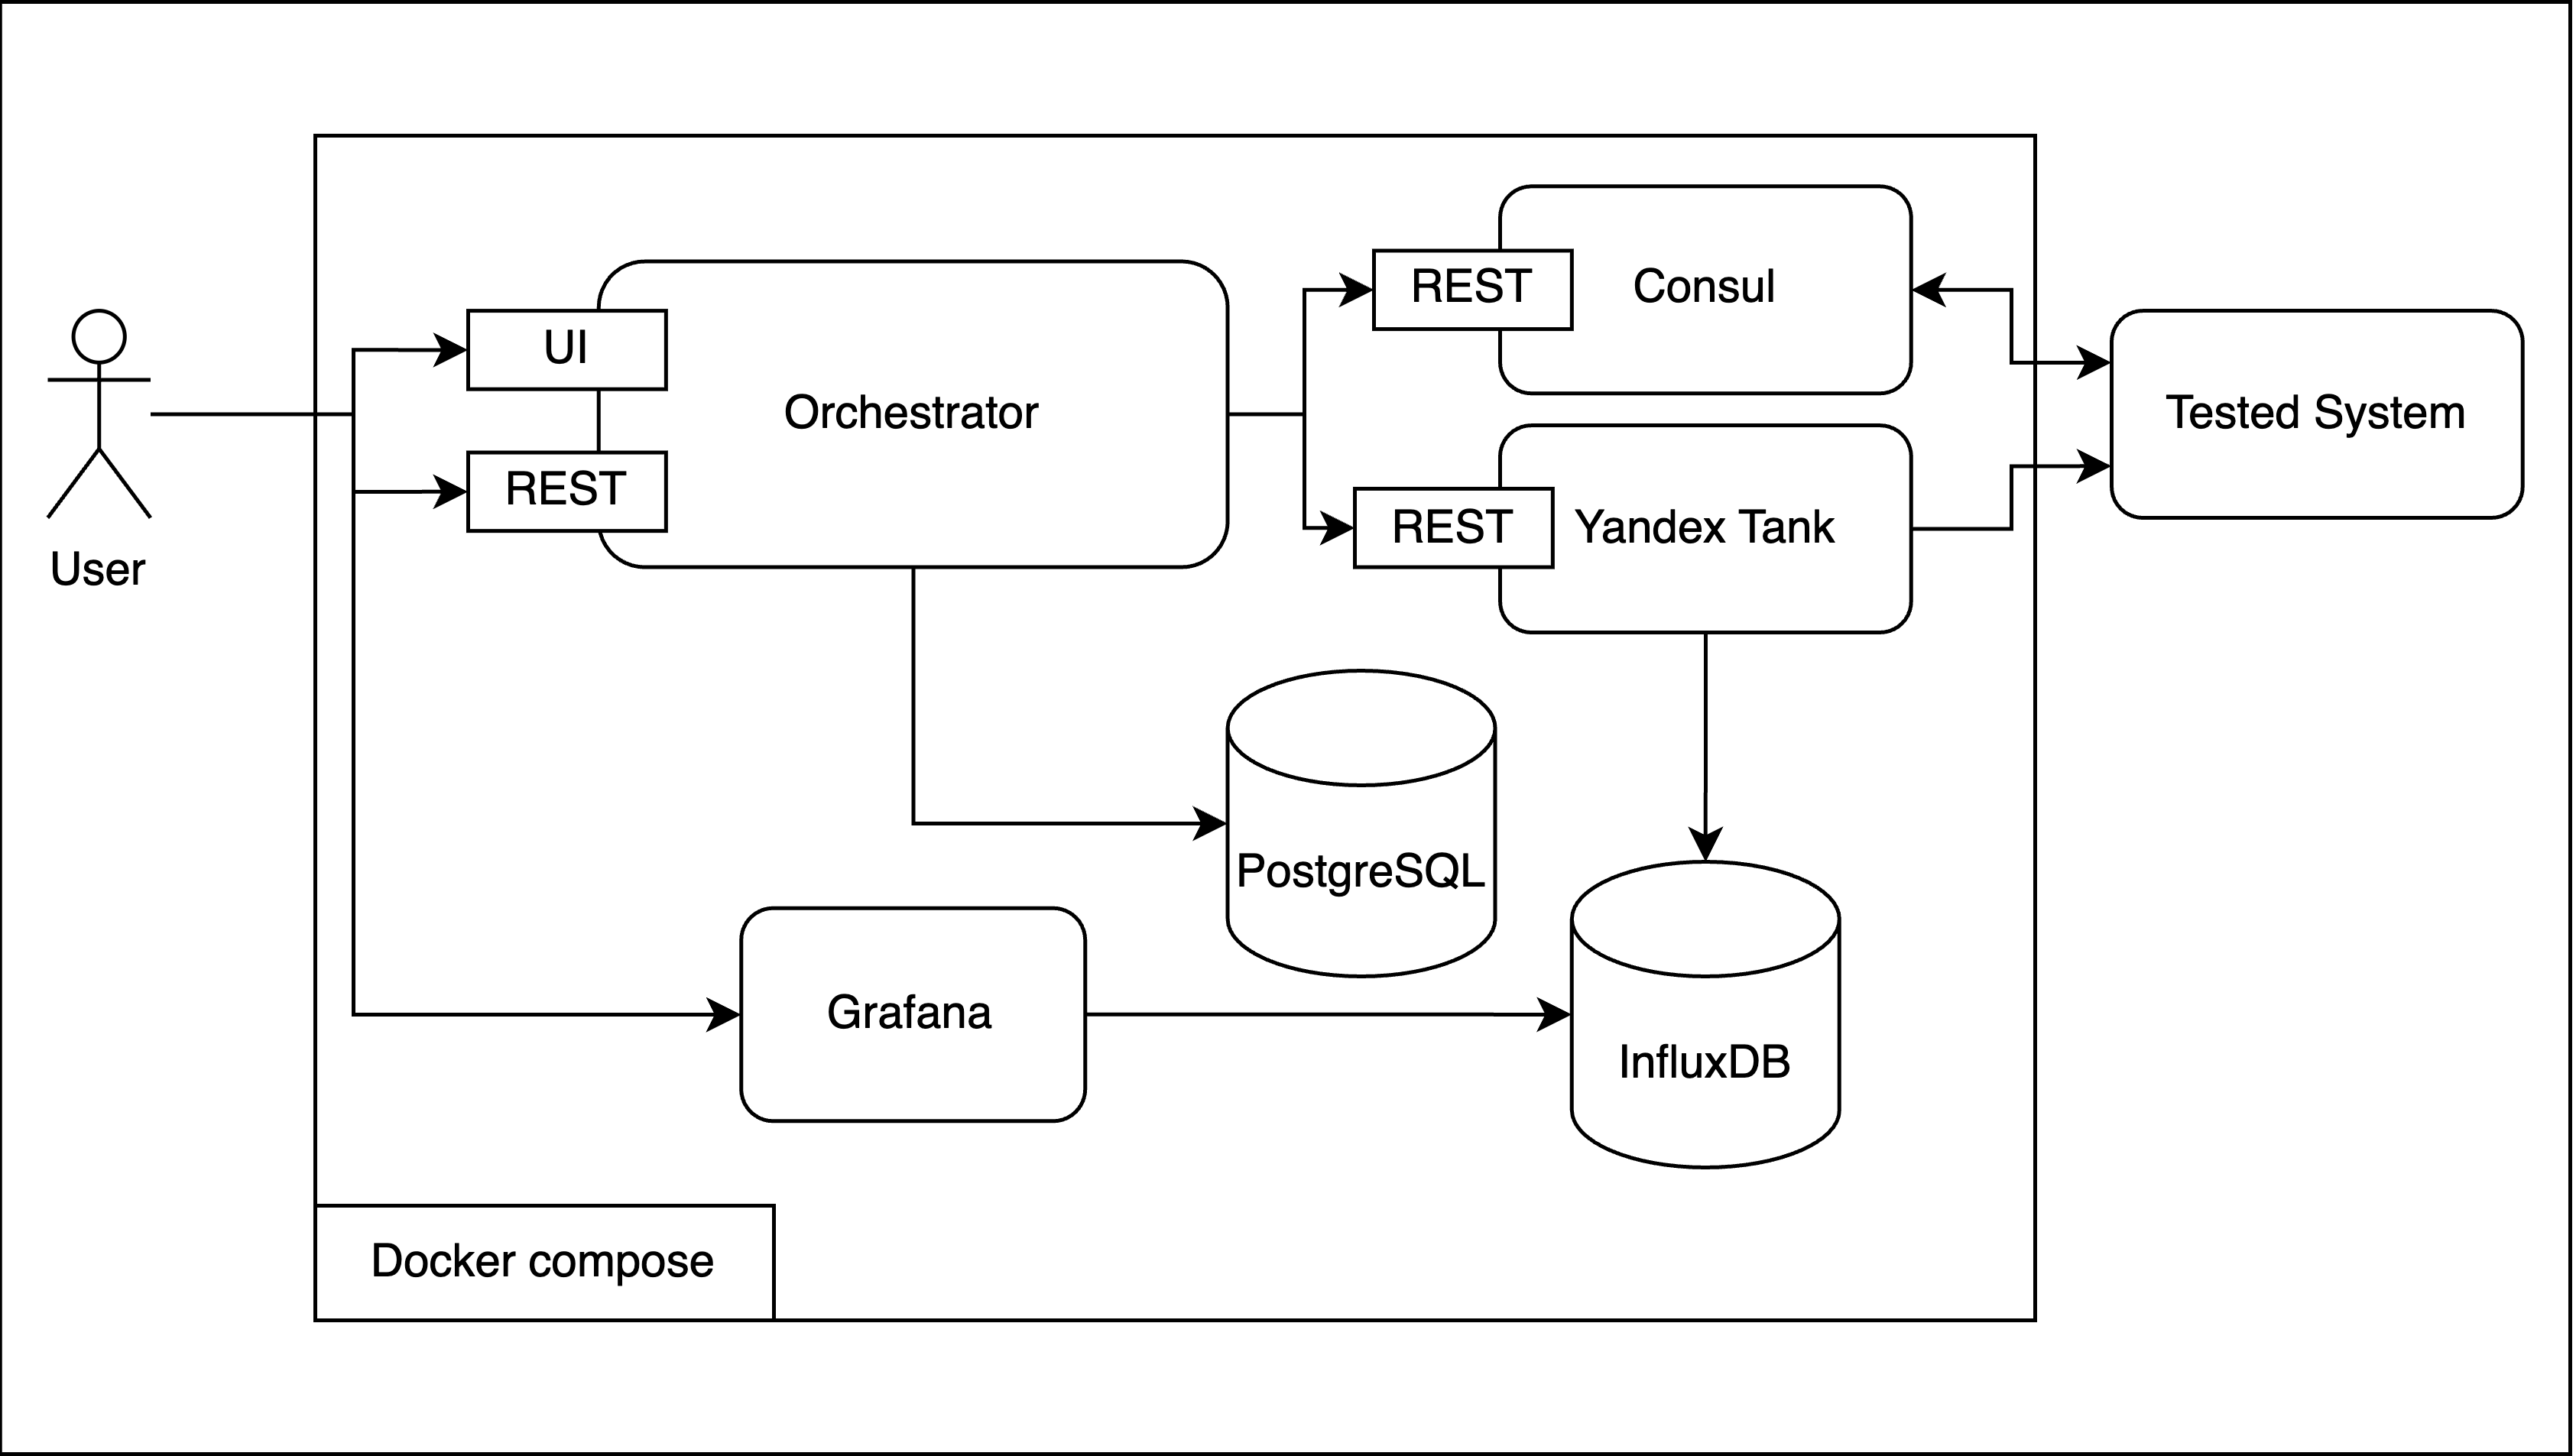
\includegraphics[height=\textheight,width=\textwidth,keepaspectratio]{architecture.png}
    \caption{Architecture of the system}
    \label{fig:architecture}
\end{figure}